\documentclass[12pt]{article}

\usepackage[english]{babel}
\usepackage{blindtext}
\usepackage{graphicx}
\usepackage{amssymb}
\usepackage{amsthm}
\usepackage{amsmath}
\usepackage{bbold}
%\textsc{•}\usepackage{bm}
%\usepackage{physics}
\usepackage[a4paper, width = 185mm, top = 15mm, bottom = 15mm]{geometry}
\usepackage{calligra}
\usepackage{float}
\usepackage{subcaption}

\DeclareMathAlphabet{\mathcalligra}{T1}{calliga}{m}{n}
\DeclareFontShape{T1}{calligra}{m}{n}{<->s*[2.2]callig15}{}

\newcommand{\scripty}[1]{\ensuremath{\mathcalligra{#1}}}
\renewcommand* \d{\mathop{}\!\mathrm{d}}



\begin{document}
\noindent
\subsection*{C++ implementation}
There is still a lot of room for improvements on the C++ implementation for the solver when it comes to scaling. But as it stands now, it's reasonbly fast and memory seems to be the clear bottleneck instead. Below is a plot that shows the speed-up of the solver and its components for 700 orbitals.
\begin{figure}[h!]
  \centering

    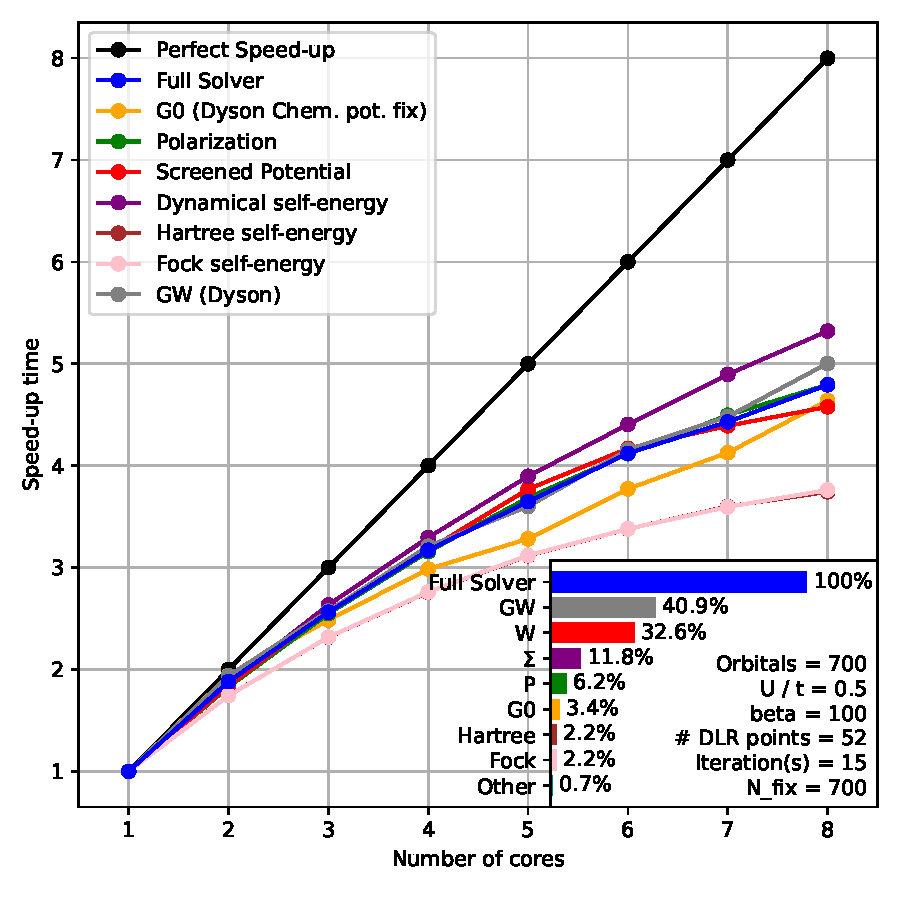
\includegraphics[width=0.53\textwidth]{700.pdf}
\end{figure}\\
The solver currently starts with a given $G_0(i\omega)$ block Green's function, it then fixes the occupation of $G_0(i\omega)$ to the desired \texttt{N\_fix} by finding the right chemical potential. With this fixed $G_0(i\omega)$, it calculates $P$, $W$, $\Sigma_\text{dyn}$, $\Sigma_\text{H}$ and $\Sigma_\text{F}$ from which it calculates a $G(i\omega)$. For the calculations above I've let the solver iterate self-consistently until the maximum difference between subsequent iterations was less than $10^{-7}$. And from what I've found, the solver seems to converege within around 15-20 iterations. (based on $U$)\\
Since we wish to consider systems with a large number of orbitals, it's clear that solving the dyson equation repeatedly to find $G(i\omega)$ along with finding the screened potential is going to take up the bulk of the time. And as for absolute times, below are some plots of the one-shot GW time and of the fully self-consistent GW time, both executed on 8 cores on my desktop.
\begin{figure}[h!]
  \centering
  \begin{subfigure}[b]{0.4\textwidth}
    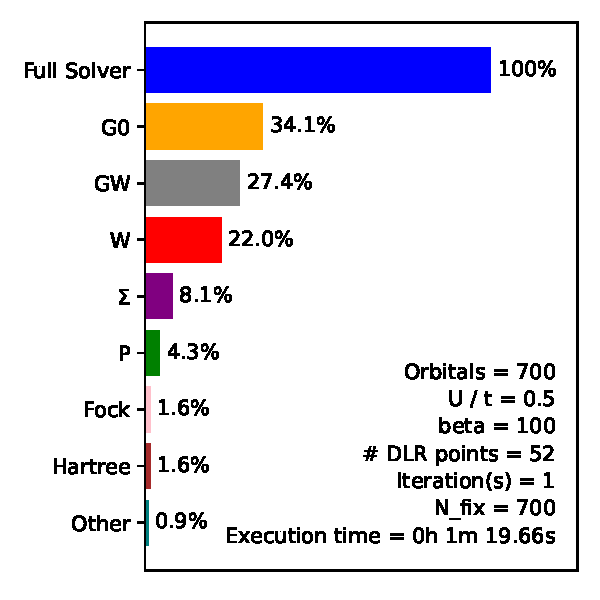
\includegraphics[width=\textwidth]{os.pdf}
    \caption{One-shot GW}
  \end{subfigure}
  \hspace{0.02\textwidth}
  \begin{subfigure}[b]{0.4\textwidth}
    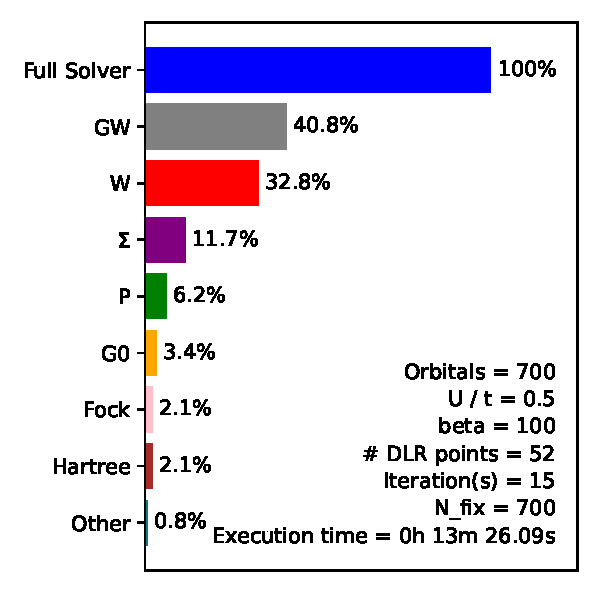
\includegraphics[width=\textwidth]{sc.pdf}
    \caption{Self-consistent GW}
  \end{subfigure}
\end{figure}\\
\newpage
\noindent
\subsection*{Back to the results of the solver}
Unless performance proves to pose an issue when considering larger systems, I think we can leave the C++ implementation for what it is at the moment. A fast solver is useless if it gives the wrong results after all.\\
From all the testing against exact diagonalization (E.D.), Pino's analytical solutions and against Hugo's implementation for the Dimer, I'm very confident the solver is giving good results. But there is still one big obstacle and that is the chemical potential and the occupation of the Green's functions. The plots below show the interacting Green's function obtained from the GW solver plotted over the results from E.D., showing only the $i=j=0$ element, the actual element being not important for what I want to show. The system is the Hubbard Dimer with only local interactions and only a one-shot GW performed.
\begin{figure}[h!]
  \centering
  \begin{subfigure}[b]{0.45\textwidth}
    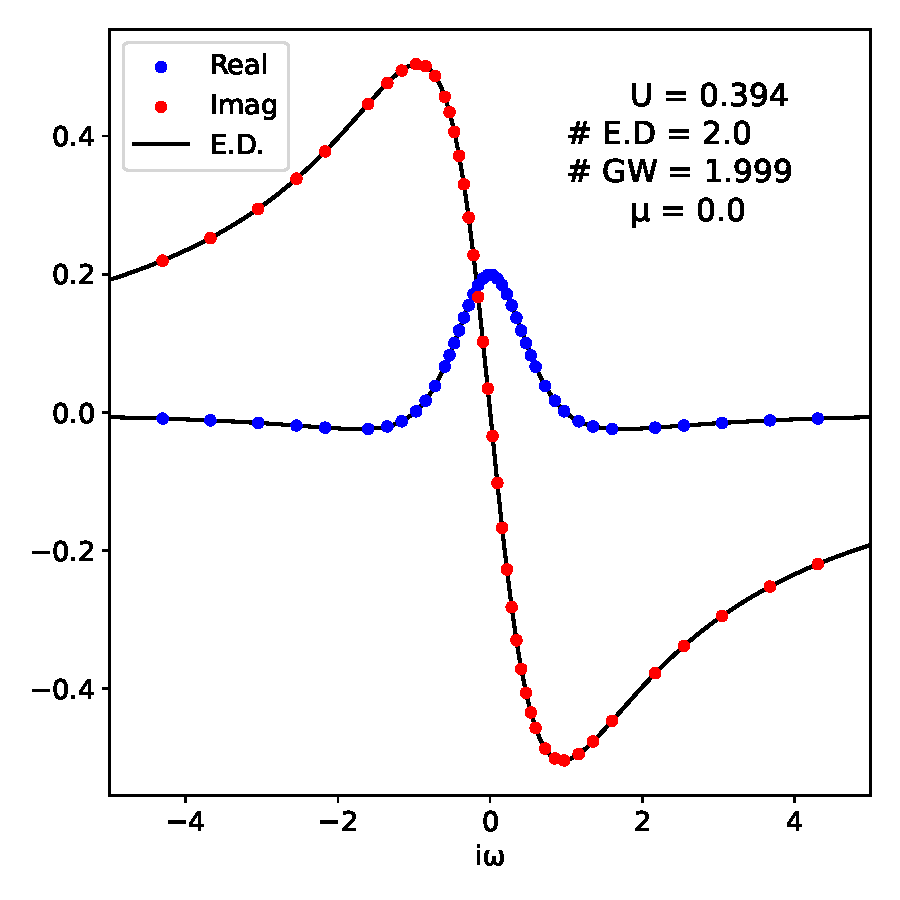
\includegraphics[width=\textwidth]{before.pdf}
    \caption{$U = 0.394$ with $\mu$ fixing for $G_0$ and $G$}
    \label{fig:sub1}
  \end{subfigure}
  \hspace{0.05\textwidth}
  \begin{subfigure}[b]{0.45\textwidth}
    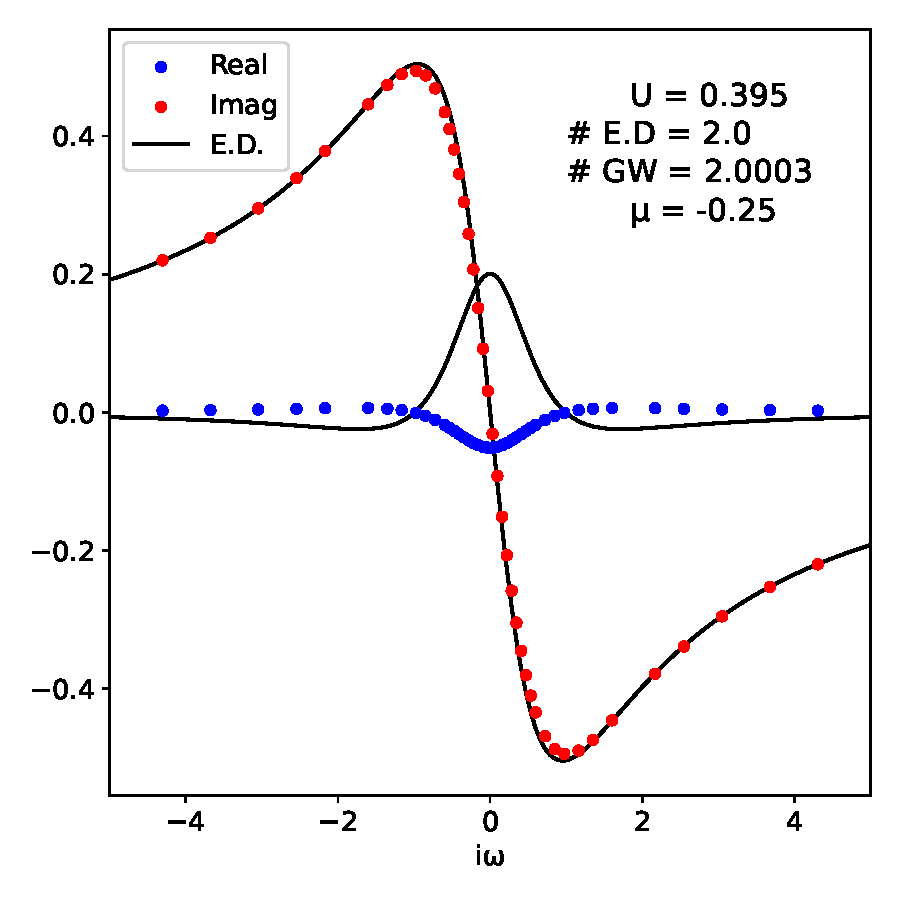
\includegraphics[width=\textwidth]{after.pdf}
    \caption{$U = 0.395$ with $\mu$ fixing for $G_0$ and $G$}
    \label{fig:sub2}
  \end{subfigure}

  \begin{subfigure}[b]{0.45\textwidth}
    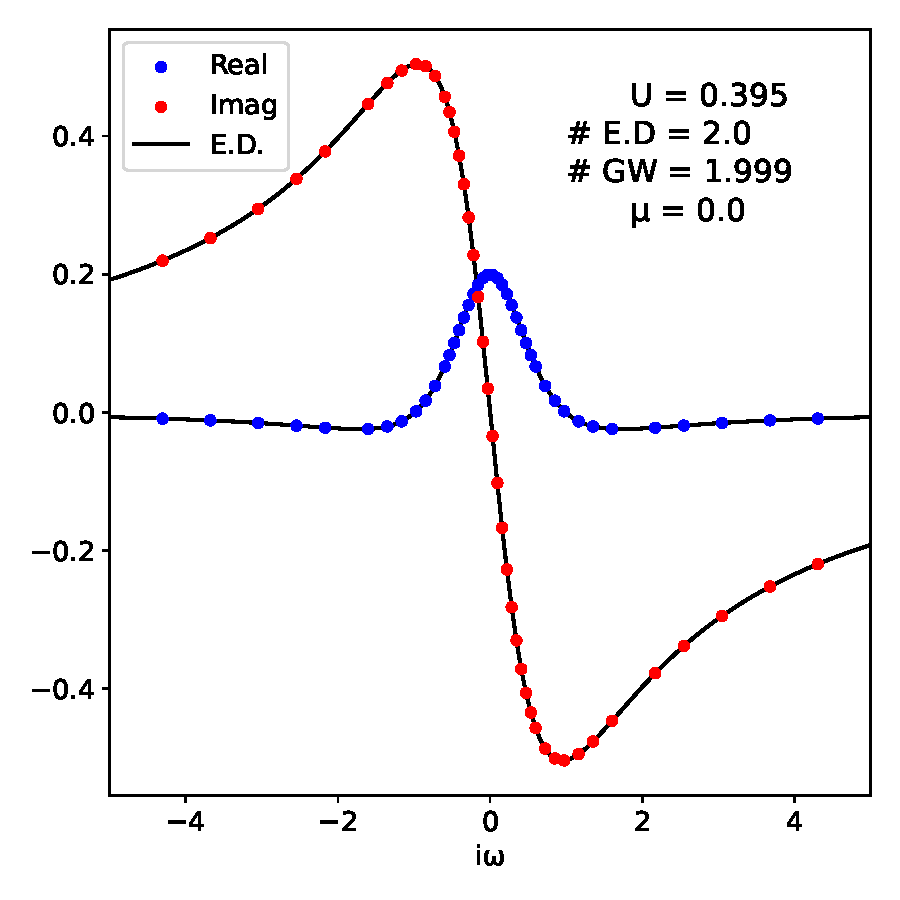
\includegraphics[width=\textwidth]{after2.pdf}
    \caption{$U = 0.395$ with $\mu$ fixing for just $G_0$}
    \label{fig:sub3}
  \end{subfigure}
  \hspace{0.05\textwidth}
  \begin{subfigure}[b]{0.45\textwidth}
    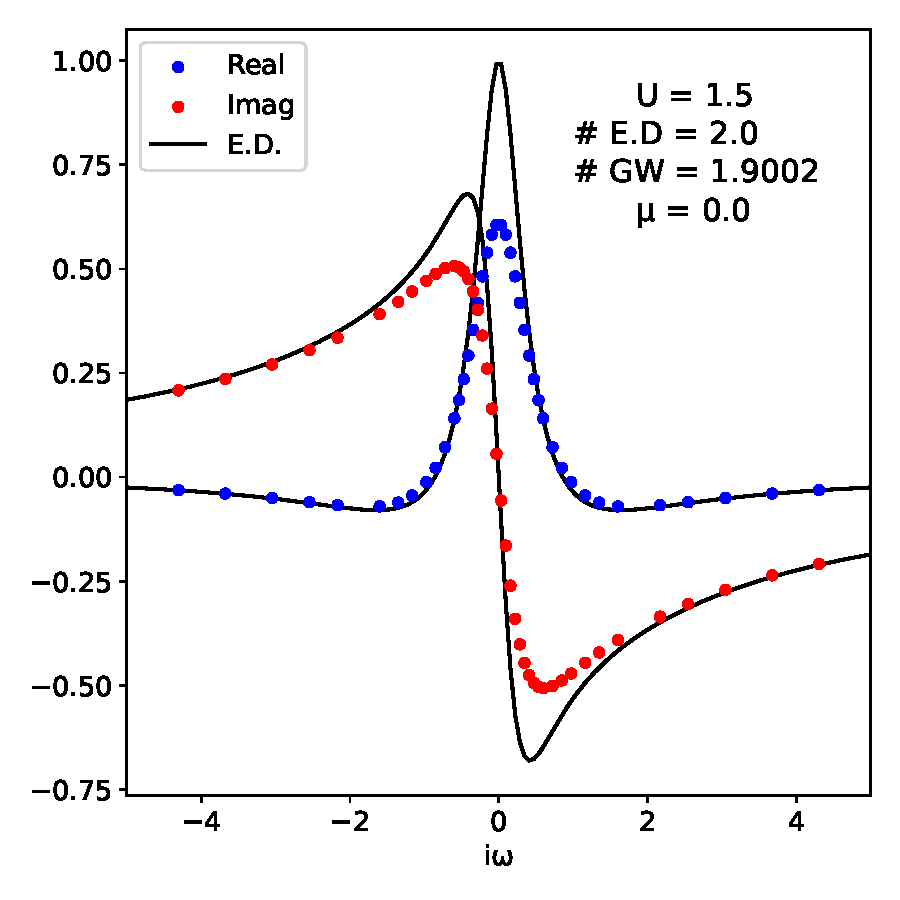
\includegraphics[width=\textwidth]{after3.pdf}
    \caption{$U = 1.5$ with $\mu$ fixing for just $G_0$}
    \label{fig:sub4}
  \end{subfigure}
\end{figure}\\
\newpage
\noindent
I supply an \texttt{N\_fix} to the solver and in subfigures (a) and (b), I fix the occupation of both the supplied $G_0$ and the found $G$ to the desired occupation. The $G_0$ made from inverting the hopping matrix is already at half filling, so $N=2$ and that's also what \texttt{N\_fix} is set to. When turning up the interactions, there is no need to change the chemical potential yet, not up to around $U=0.394$ in this case. There is nothing special about this value for $U$, it's just the value at which the occupation of $G$ dips below the set threshold \texttt{N\_tol} which is set to $10^{-3}$ and thus the chemical potential fixer does its job and shifts the chemical potential as seen in (b). Here $\mu$ for $G$ has been found to be $-0.25$ but as we can see, there is a large change in the results.\\
If instead, we ignore the chemical potential fixing for $G$ as shown in (c), we actually get our sensible results again that agrees with E.D. (which is fixed to \texttt{N\_fix}). We can even increase the interaction strength much higher as seen in (d). Here the occupation of $G$ is definitely wrong, but the result still somewhat agrees with E.D.\\
One might perhaps wonder that this is caused by the sudden increase in $\mu$, it goes from 0 to -0.25 at just a small change in $U$. I can adjust the chemical potential finder to use step sizes based on the difference between the occupation and the desired occupation and this fixes the sudden jump, but it still gives wrong results with increasing $U$ and if \texttt{N\_tol} is set any lower, we get these sudden jumps regardless.\\
\\
The solver seems to give the best results when the chemical potential is not fixed to a desired occupation. 
\subsection*{Self-consistent GW}
Something interesting happens if we start iterating inside the solver. In subfigure (d) we could see that GW somewhat agreed with E.D. if we didn't fix the chemical potential but our occupation was $\sim 1.9$ instead of 2. But if we left the solver iterate until self-consistency, the occupation actually goes back up to 2. Below is a plot of the GW result which iterated 20 times:
\begin{figure}[h!]
\centering
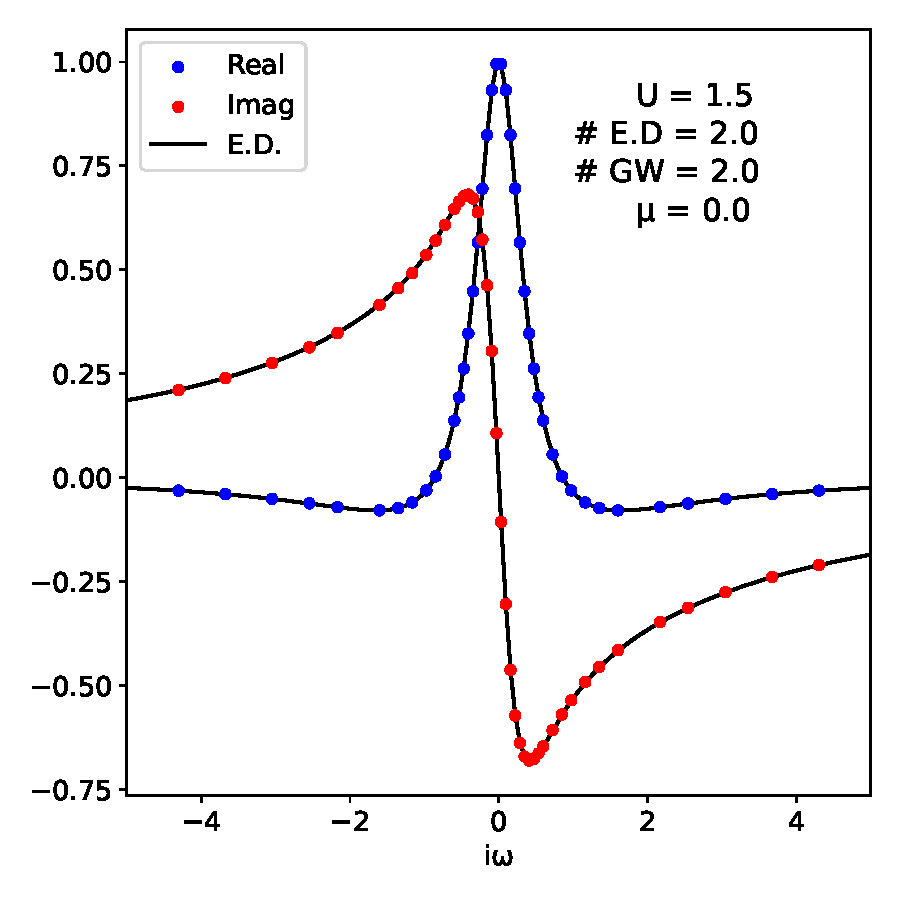
\includegraphics[width=0.6\textwidth]{sc2.pdf}
\end{figure}\\
So letting the solver iterate seems to be the way to get better results. There is now also no need for chemical potential fixing as the occupation matches the desired one already. But there are still some issues which I'll touch upon later.
\newpage
\noindent
\subsection*{Something about the errors}
The scatter plots are nice, but real numbers give a clearer picture. Below is a plot that shows the maximum relative error between the GW result and E.D. for the Hubbard dimer as the interaction strength is turned up. It also shows the trend for a different number of total interations:
\begin{figure}[h!]
\centering
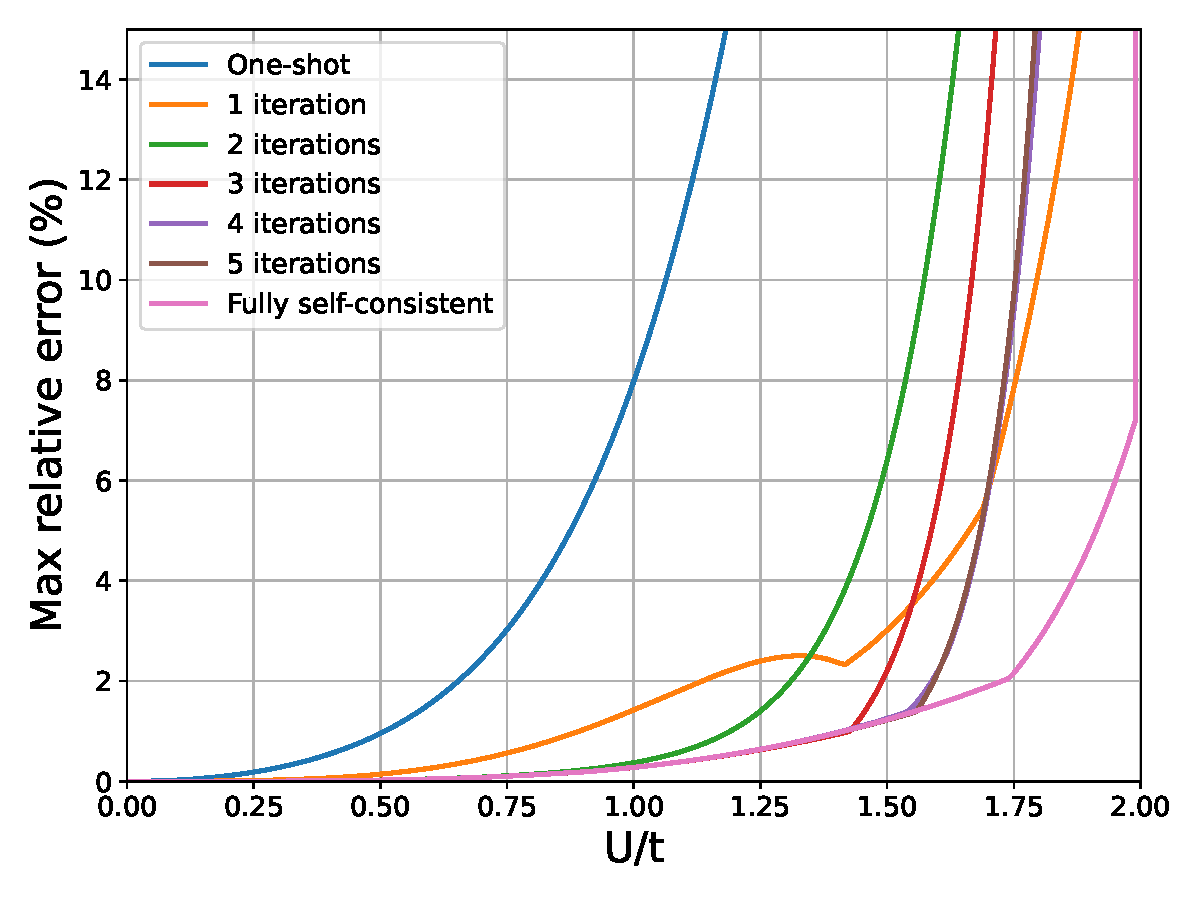
\includegraphics[width=0.6\textwidth]{errors2.pdf}
\end{figure}\\
Even with $U$ definitely greater than $t$, the solver still gives very good results with maximum relative errors on the order of less than 2\% up to $U=1.75$. But there is clearly something that happens at $U = 2$ with the solver never being self-consistent.\\
Below is the same plot repeated for 4 sites at half filling:
\begin{figure}[h!]
\centering
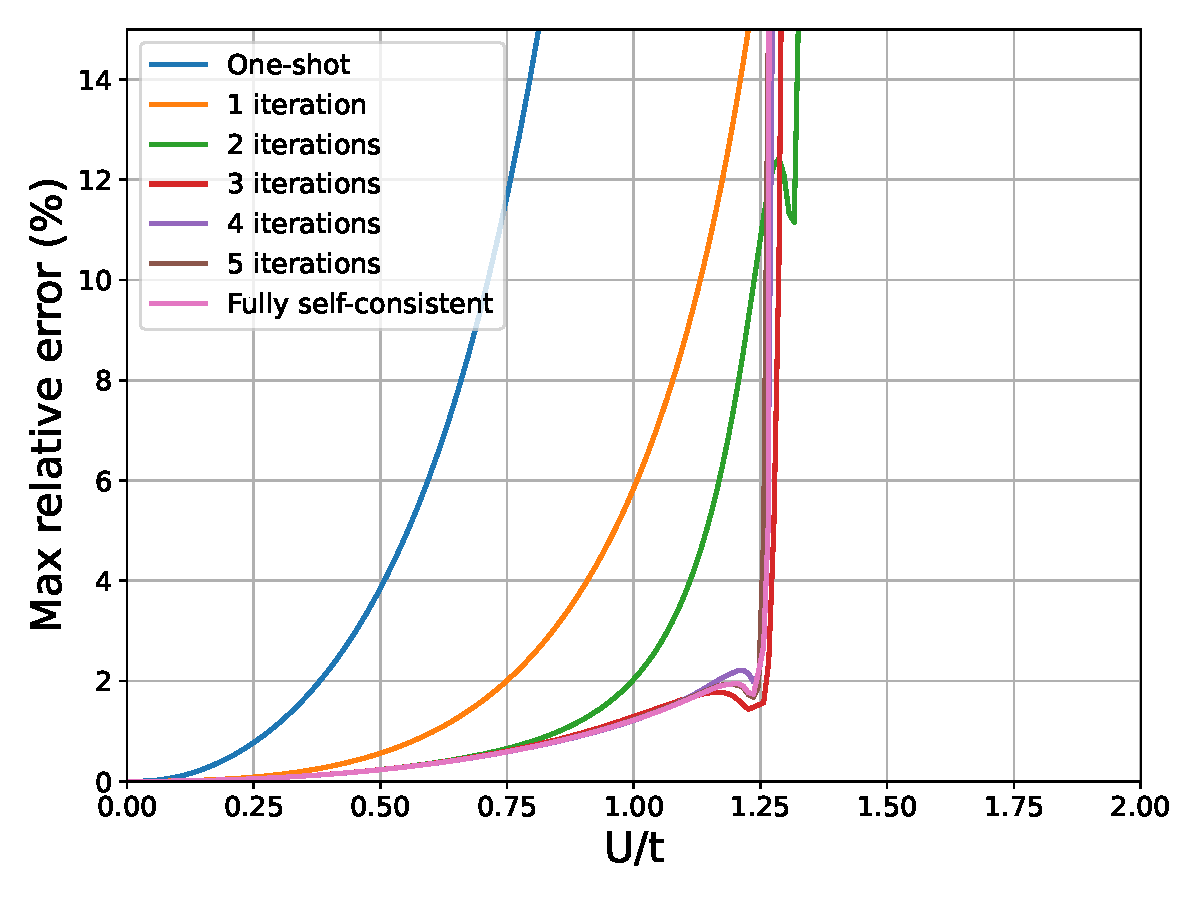
\includegraphics[width=0.6\textwidth]{errors4.pdf}
\end{figure}\\
Again, it seems like the max relative error is below 2\% but now something happens at $U\sim 1.25$.\\
\\
Could these be phase transitions of sorts? Something that E.D. does capture but GW completely fails to do so?
\newpage
\noindent
\subsection*{Issues with occupation}
As it stands, the solver seems to work pretty well for half filling. Here the constructed $G_0$ is already at the correct occupation so there is no need to fix the chemical potential of $G_0$ and after iterating self consistently, $G$ is also at the same occupation. But this only works for an even number of orbitals. Below are plots of the occupation against the chemical potential.
\begin{figure}[h!]
  \centering
  \begin{subfigure}[b]{0.45\textwidth}
    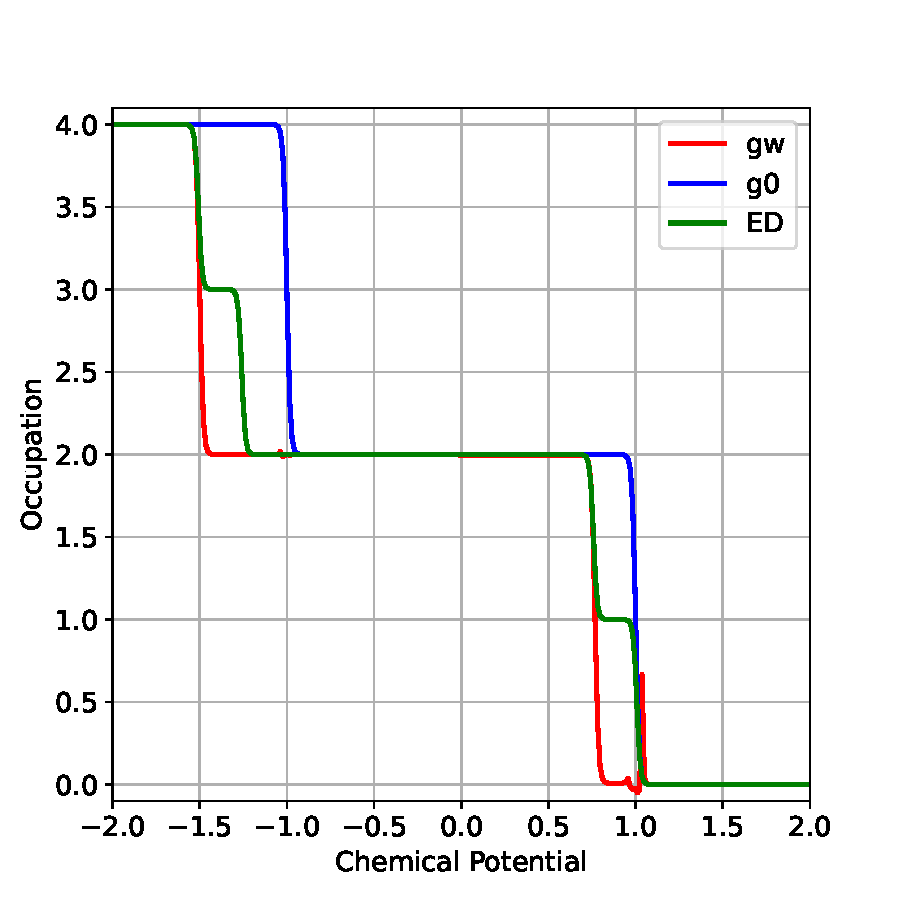
\includegraphics[width=\textwidth]{o2.pdf}
    \caption{2 orbitals, $U=0.5$}
  \end{subfigure}
  \hspace{0.02\textwidth}
  \begin{subfigure}[b]{0.45\textwidth}
    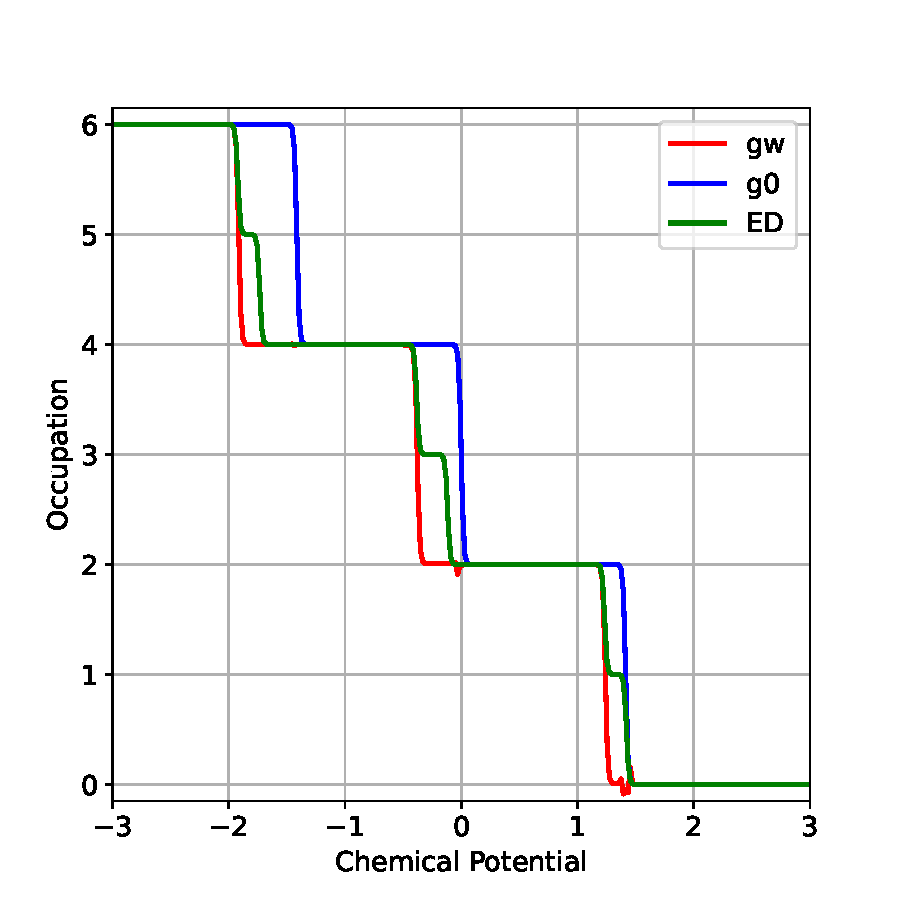
\includegraphics[width=\textwidth]{o3.pdf}
    \caption{3 orbitals, $U=0.5$}
  \end{subfigure}
\end{figure}\\
The line for $G_0$ is obtained by inverting the hopping matrix with the given potential and then finding the occupation. The line for E.D. is obtained by adding the chemical potential times the particle number operator to the Hamiltonian and the line for $G$ is obtained by simply performing the GW solver and not adjusting the chemical potential any further, so just starting with a $G_0$ at that given chemcial potential.\\
\\
What we can see is that the interactions cause a shift in the graph compared to the non-interacting case. For an even number of orbitals, this doesn't matter too much because we'll remain at the correct occupation as seen by the plateau. But for an odd number of occupation, the shift means that for zero chemical potential, we actually move down one occupation, both for GW and E.D. And say we look at (a), if we were to fix the occupation of $G_0$ to 3, $G$ would still be at 2 because of the shift.\\
This means that I get agreeing results for an even number of orbitals if I fix the chemical potential. This also works for cases besides half filling, but only if the occupation is still an even number. For odd occupations I get the best results by not fixing the chemical potential at all, but then I do end up at the wrong occupation for both GW and E.D..\\
And I think the fact that we struggle with odd occupations could be because GW doesn't actually have a step at odd occupations like E.D. does.



\end{document}